\begin{frame}
    \frametitle{Arquitectura de Control}
    \note{Información extraída de https://youtu.be/pEVsedl2KO4?si=_cwQpRPPUnQ04B3c}
    
    \begin{center}
        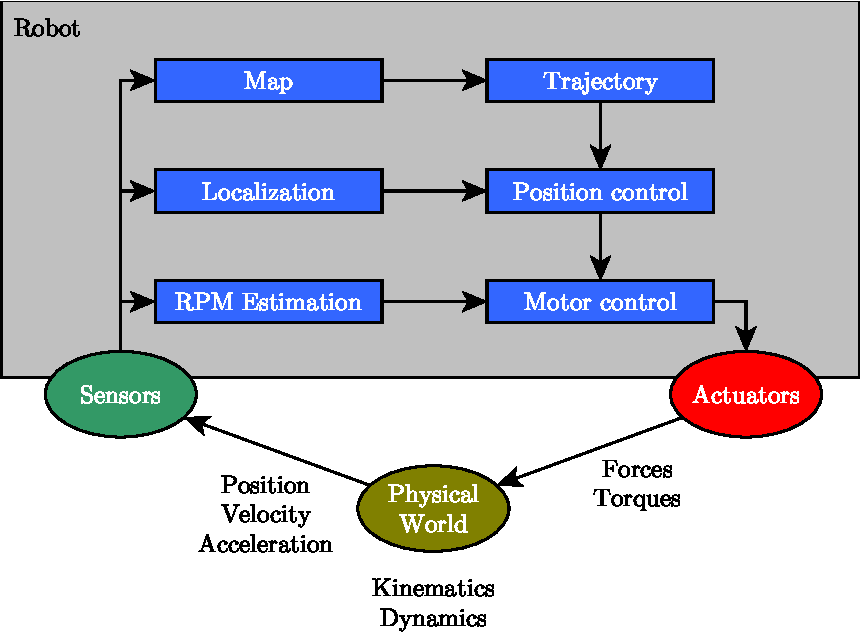
\includegraphics[width=0.7\columnwidth]{./images/control_architecture.pdf}
    \end{center}
    

    \note{En la literatura también se lo denomina think-act-sense paradigm}
        
    \note{La caja gris representa el software de navegación del robot. En la literatura, a esta parte se la denomina thinking}
    
    \note{En la literatura también se llamada a la parte de los actuadores acting}
    
    \note{En la literatura a la parte de los sensores se la denomina sensing}
    
    \note{Control a nivel de trayectoria: se debe garantizar seguir a la trayectoria deseada de manera suave}
    \note{Control a nivel de posicionamiento: se debe garantizar que se alcanza un punto en la trayectoria que se desea realizar.}
    \note{Control a nivel de actuadores (motores): para controlar la velocidad de los motores de las ruedas.}
    
   
\end{frame}
